\section{Mapping Rules for RDF: Conceptual Mapping}
\label{sec:chp4_cm_ontology}

Based on the analysis performed in \cref{sec:chp4_framework}, we abstract the features and limitations present in current mapping languages to represent them in an ontology. This ontology aims at gathering the expressiveness of current mapping languages, and is called the Conceptual Mapping\footnote{\label{foot:cmportal}\url{https://w3id.org/conceptual-mapping/portal}}. The methodology followed to build this ontology is first presented, and then each step of its construction is described in detail.

\subsection{Methodology}
The Conceptual Mapping ontology was developed following the guidelines provided by the Linked Open Terms (LOT) methodology. LOT is a well-known and mature lightweight methodology for the development of ontologies and vocabularies that has been widely adopted in academic and industrial projects~\citep{poveda2022lot}. It is based on the previous NeOn methodology~\citep{suarez2015neon} and includes four major stages: Requirements Specification, Implementation, Publication, and Maintenance~\cref{fig:lot}. In this section, we describe these stages and how they have been applied and adapted to the development of the Conceptual Mapping ontology.

\noindent\textbf{Requirements specification}
This stage refers to the activities carried out for defining the requirements that the ontology must meet. At the beginning of the requirements identification stage, the goal and scope of the ontology are defined. Following, the domain is analyzed in more detail by looking at the documentation, data that has been published, standards, formats, etc. In addition, use cases and user stories are identified. Then, the requirements are specified in the form of competency questions and statements. 

In this case, the specification of requirements includes purpose, scope, and requirements. The requirements are specified as facts rather than competency questions and validated with Themis~\citep{fernandez2021themis}, an ontology evaluation tool that allows validating requirements expressed as tests rather than SPARQL queries. We consider this approach to be adequate in this case since (1) there are no use cases as this ontology is a mechanism of representation of  mapping language's features; and (2) there are no SPARQL queries because they result from Competency Questions which are in turn extracted from use cases and user stories. Further details are shown in \cref{sec:chp4_requirements}.

\noindent\textbf{Implementation}
The goal of the Implementation stage is to build the ontology using a formal language, based on the ontological requirements identified in the previous stage. From the set of requirements a first version of the model is conceptualized. The model is subsequently refined by running the corresponding evaluations. Thus, the implementation process follows iterative sprints; once it passes all evaluations and meets the requirements, it is considered ready for publication.

The conceptualization is carried out representing the ontology in a graphical language using the  Chowlk notation~\citep{feria2022chowlk} (as shown in \cref{fig:cm_diagram}). The ontology is implemented in OWL 2 using Protégé. The evaluation checks different aspects of the ontology: (1)  requirements are validated using  Themis~\citep{fernandez2021themis}, (2)  inconsistencies are found with the Pellet reasoner, (3)  OOPS!~\citep{poveda2014oops} is used to identify modeling pitfalls, and (4) FOOPS!~\citep{garijo2021foops} is run to check the FAIRness of the ontology. Further details are described in \cref{sec:chp4_implementation}.

\noindent\textbf{Publication}
The publication stage addresses the tasks related to making the ontology and its documentation available. The ontology documentation was generated with Widoco~\citep{garijo2017widoco}, a built-in documentation generator in OnToology~\citep{alobaid2019automating}, and it is published with a W3ID URL\footnote{\label{foot:cmlink}\url{https://w3id.org/conceptual-mapping}}. The ontology and related resources can be accessed in the ontology portal. Further details are presented in \cref{sec:chp4_pub-main}.
%The ontology is published using a persistent URL \footnote{\url{https://w3id.org/conceptual-mapping}}.  and HTML documentation was generated with Widoco~\citep{garijo2017widoco}, using OnToology~\citep{alobaid2019automating}. As for maintenance, the ontology is available in a GitHub repository \footnote{https://github.com/oeg-upm/Conceptual-Mapping}.

\begin{figure}[!t]
\centering
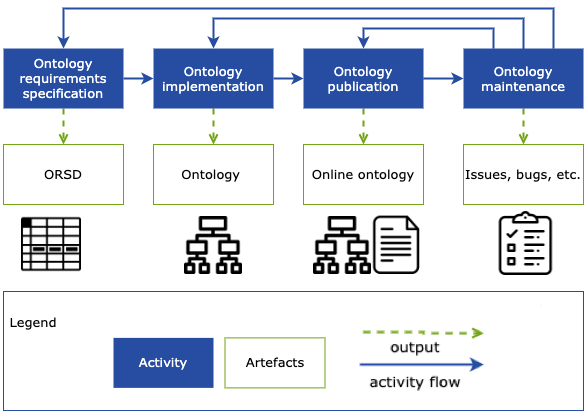
\includegraphics[width=0.6\linewidth]{figures/lot.png}
\caption{Workflow proposed by the LOT Methodology~\citep{poveda2022lot}.}
\label{fig:lot}
\end{figure}

\noindent\textbf{Maintenance}

Finally, the last stage of the development process, maintenance, refers to ontology updates as new requirements are found and/or errors are fixed. The ontology presented in this work promotes the gathering of issues or new requirements through the use of issues in the ontology GitHub repository. Additionally, it provides control of changes, and the documentation enables access to previous versions. Further details are shown in \cref{sec:chp4_pub-main}.



\subsection{Requirements}
\label{sec:chp4_requirements}

This section presents the purpose, scope, and requirements of the Conceptual Mapping Ontology. In addition, it also describes from where and how the requirements are extracted: analysing the mapping languages (presented as a comparative framework in \cref{sec:chp4_framework}) and the Mapping Challenges proposed by the community.

\subsubsection{Purpose and scope}

The Conceptual Mapping ontology aims at gathering the expressiveness of declarative mapping languages that describe the transformation of heterogeneous data sources into RDF. This ontology-based language settles on the assumption that all mapping languages used for the same basic purpose of describing data sources in terms of an ontology to create RDF, must share some basic patterns and inherent characteristics. Inevitably, not all features are common. As described in previous sections, some languages were developed for specific purposes, others extend existing languages to cover additional use cases, and others are in turn based in languages that already provide them with certain capabilities. The Conceptual Mapping ontology is designed to represent and articulate these core features, which are extracted from two sources: (1) the analysis of current mapping languages, and (2) the limitations of current languages identified by the community. These limitations, proposed by the W3C Knowledge Graph Construction Community Group\footnote{\label{foot:kgc}\url{https://www.w3.org/community/kg-construct/}}, are referred to as Mapping Challenges\footnote{\label{foot:challenges}\url{https://w3id.org/kg-construct/workshop/2021/challenges.html}} and have been partially implemented by some languages. %Both sources are described throughout this section.

This ontology also presents some limitations. As shown in \cref{sec:chp2_mappings}, mapping languages can be classified into three categories according to the schema in which they are based: RDF-based, SPARQL-based and based on other schemes. The Conceptual Mapping is included in the first category and, as such, has the same inherent capabilities and limitations as RDF-based languages regarding the representation of the language as an ontology. This implies that it is feasible to represent their expressiveness, whereas reusing classes and/or properties or creating equivalent constructs. Languages based on other approaches usually follow schemas that make them relatable to ontologies. This can be seen in the correspondence between YARRRML and RML: RML is written in Turtle syntax. YARRRML~\citep{Heyvaert2018yarrrml} is mainly used as a user-friendly syntax to facilitate the writing of RML rules. It is based on YAML, and can easily be translated into RML\footnote{\url{https://rml.io/yarrrml/matey/}}. 

Lastly, SPARQL-based languages pose a challenge. SPARQL is a rich and powerful query language~\citep{perez2009semantics} to which these mapping languages add more capabilities (e.g., SPARQL-Generate, SPARQL-Anything). It has an innate flexibility and capabilities sometimes not comparable to the other languages. For this reason, representing every single capability and feature of SPARQL-based languages is out of the scope of this work. Given the differences of representation paradigm between RDF and SPARQL for creating mappings, it cannot be ensured that the Conceptual Mapping covers all possibilities that a SPARQL-based language can, and as such, is considered a limitation.


\subsubsection{Mapping Challenges}
\label{sec:chp4_mapping_challenges}

Following its inception, the W3C Knowledge Graph Construction Community Group\cref{foot:kgc} defined a series of challenges for mapping languages based on the experience of members in using declarative mappings\cref{foot:challenges}. These challenges are a summary of the limitations of current languages. They have been partially addressed independently in some of the analyzed languages, such as RML~\citep{delva2021rml-fields} and ShExML~\citep{garcia2021shexml-challenges}. These challenges are summarized as follows:

\begin{itemize}
    \item \textbf{[C1] Language Tags and Datatype.} It refers to dynamically building language tags ([C1a]) and datatypes ([C1b]), that is, from data rather than as constant values.
    \item \textbf{[C2] Iterators.} This challenge addresses the need to access data values 'outside' the iteration pattern ([C2a]), especially in \textcolor{black}{some tree-like data sources such as JSON}; and iterating over multi-value references ([C2b]).
    \item \textbf{[C3] Multi-value References.} It discusses how languages  handle data fields that contain multiple values ([C3a]), their datatypes and associated language tags ([C3b]).
    \item \textbf{[C4] RDF Collections and Containers.} This challenge addresses the need to handle RDF collections and containers.
    \item \textbf{[C5] Joins.} It refers to joining resources with zero join conditions ([C5a]) and joining literals instead of IRIs ([C5b]).
\end{itemize} 


\subsubsection{Conceptual Mapping Requirements}

In order to extract the requirements that serve as the basis for the development of the Conceptual Mapping ontology, we take as input the analysis from the comparison framework (\cref{sec:chp4_framework}) and the Mapping Challenges (\cref{sec:chp4_mapping_challenges}) described previously and the expertise of the authors. From a combination of their features, we extract 30 requirements. These requirements are expressed as facts, and are available in the ontology repository and portal\footnote{\url{https://oeg-upm.github.io/Conceptual-Mapping/requirements/requirements-core.html}}. Each requirement has a unique identifier, its provenance (comparison framework or mapping challenge id) and the corresponding constructs in the ontology. The constructs are written in Turtle, and lack cardinality restrictions for the sake of understandability. These requirements are tested with Themis, and its corresponding tests include these restrictions. More details on the evaluation of the requirements are provided in \cref{sec:eval}. 

The requirements gathered range from general-purpose to fine-grained details. The general-purpose requirements refer to the basic fundamental capabilities of mappings, e.g., to create the rules to generate RDF triples (cm-r8) from reference data sources (cm-r7). The requirements with the next level of detail involve some specific restrictions and functionalities, e.g. to indicate the specific type (whether they are IRIs, Blank nodes, etc.) of subjects (cm-r16), predicates (cm-r17), objects (cm-r18), named graphs (cm-r19), datatypes (cm-r20) and language tags (cm-r21); the possibility of using linking conditions (cm-r23) and functions (cm-r15). Finally, some requirements refer to specific details or features regarding the description of data sources (e.g. cm-r4, cm-r6) and transformation rules (e.g. cm-r14, cm-r22, cm-r25).

Not all the observed features in the comparison framework have been added to the set of requirements. Some features are really specific, and supported by a minority of languages, sometimes only one language. As a result, we selected the (really) detailed features in these requirements to build the core specification of the Conceptual Mapping when they tackled the basic functionalities of the language. The rest of the details are left to be included as extensions. This differentiation and the modeling criteria is explained further in \cref{sec:chp4_implementation}.










\subsection{Implementation}
\label{sec:chp4_implementation}

This section describes in detail the activities and tasks carried out to implement the ontology, that consists in the conceptualization of the model, the encoding in a formal language, and the evaluation to fix errors, inconsistencies, and ensure that it meets the requirements. Additionally, an example of the ontology's use is presented at the end of the section.



\subsubsection{Ontology Conceptualization}




\begin{sidewaysfigure*}[]
    \centering
    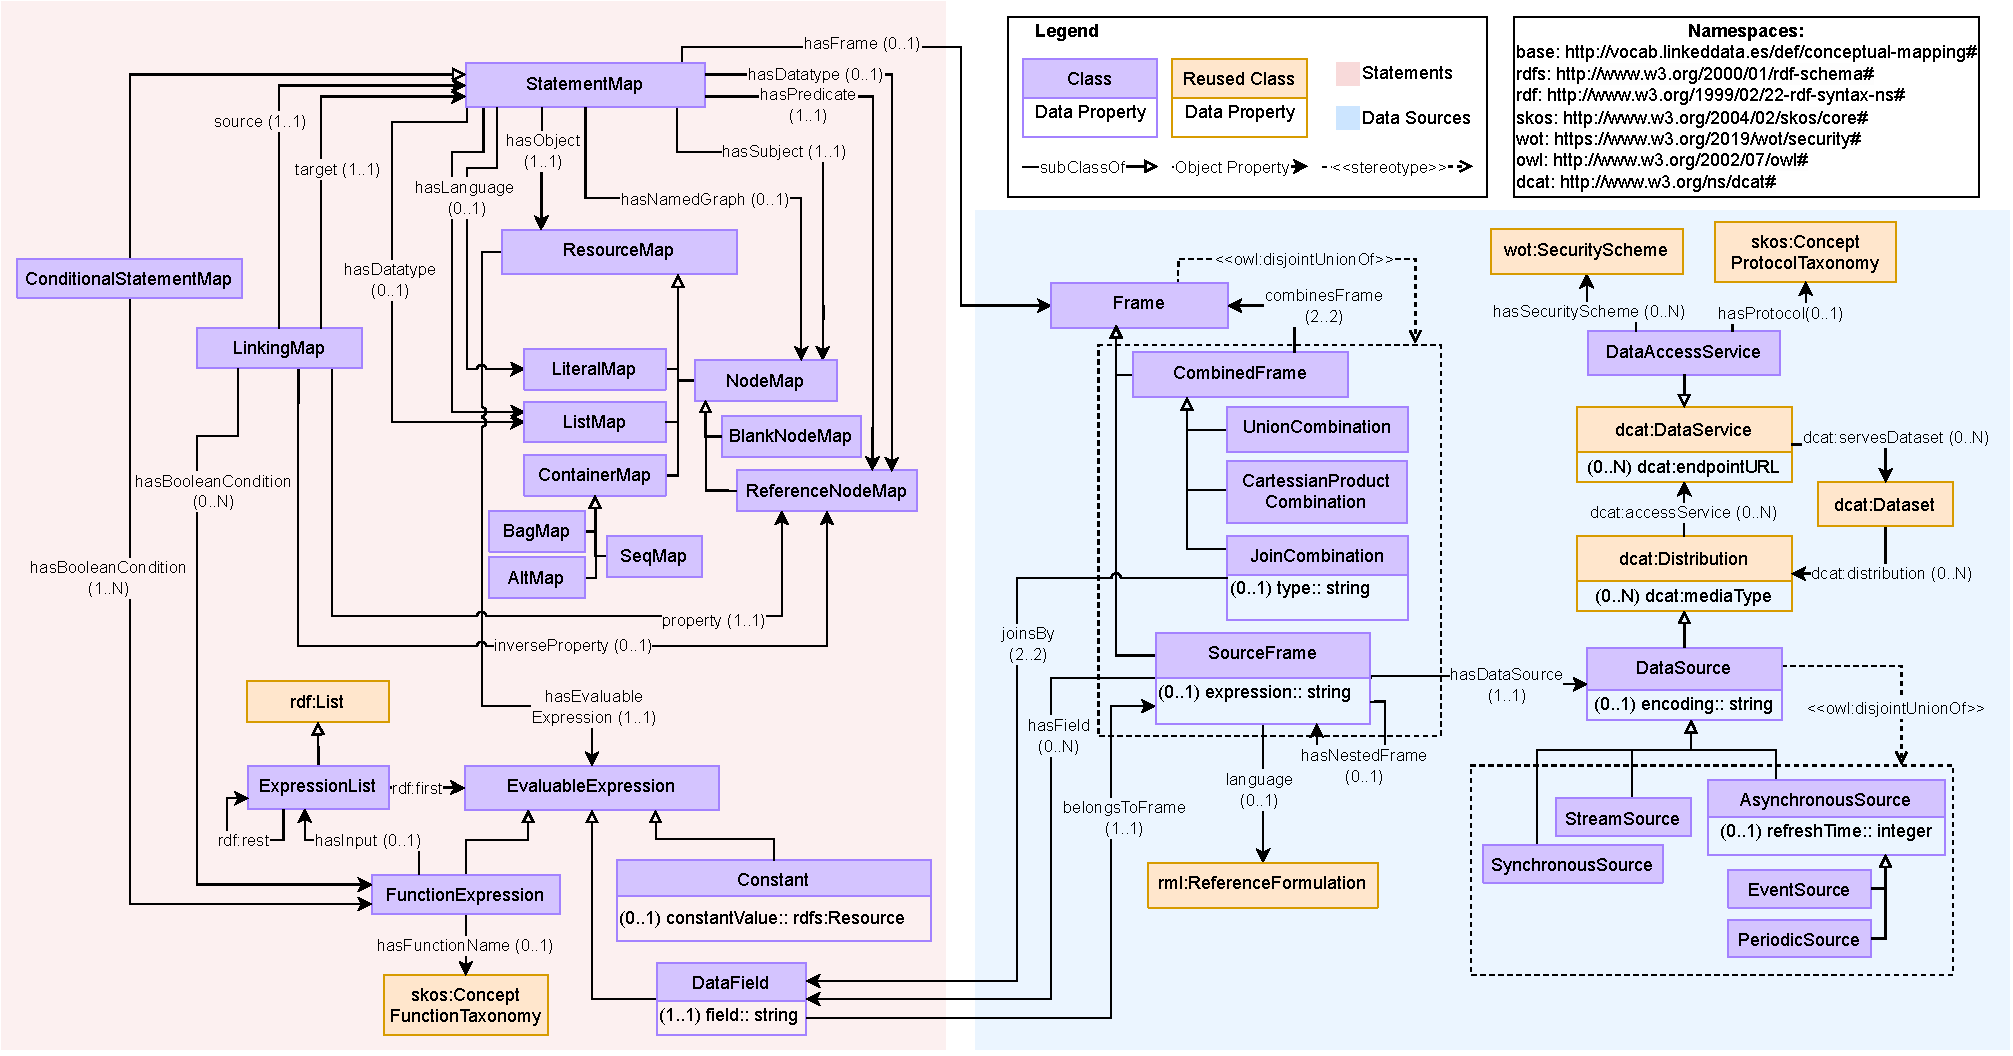
\includegraphics[width=1\linewidth]{figures/cm_diagram}
    \caption{Visual representation of the Conceptual Mapping ontology created using the Chowlk diagram notation~\citep{feria2022chowlk}.}
    \label{fig:cm_diagram}
\end{sidewaysfigure*}

\textcolor{black}{The ontology's conceptualization is built upon the requirements extracted from experts experience, a thorough analysis of the features and capabilities of current mapping languages presented as a comparative framework; and the languages' limitations discussed by the community and denoted as Mapping Challenges. The resulting ontology model is depicted in \cref{fig:cm_diagram}. This model represents the core specification of the Conceptual Mapping ontology that contains the essential features to cover the requirements. Some detailed features are also included when considered important to the language expressiveness, or needed for the language main functionality. Other detailed features are considered as extensions, as explained further in this section \ana{ojo las extensiones}. For description purposes, we divide the ontology into two parts, \textit{Statements} and \textit{Data Sources}, that compose the core model. These two parts, when not used in combination, cannot describe a complete mapping. For that reason they are not separated into single modules. } 

\noindent\paragraph{\textbf{Data sources.}} A data source (\texttt{DataSource}) describes the source data that will be translated. For this section, the Data Catalog (DCAT) vocabulary~\citep{albertoni2020dcat2} has been reused. \texttt{DataSource} is a subclass of \texttt{dcat:Distribution}, which is a specific representation of a dataset (\texttt{dcat:Dataset}), defined as ``data encoded in a certain structure such as lists, tables and databases''. A source can be a streaming source (\texttt{StreamSource}) that continuously generates data, a synchronous source (\texttt{SynchronousSource}) or an asynchronous source (\texttt{AsynchronousSource}). Asynchronous sources, in turn, can be event sources (\texttt{EventSource}) or periodic sources (\texttt{Periodic Source}). The details of the data source access are represented with the data access service class (\texttt{Data AccessService}), which in turn is a subclass of \texttt{dcat:DataService}. This class represents a collection of operations that provides access to one or more datasets or data processing functions, i.e., a description of how the data is accessed and retrieved. The data access service optionally has a security scheme (e.g., OAuth2, API Key, etc.) and an access protocol (e.g., HTTP(s), FTP, etc.).

Data properties in the \texttt{dcat:Dataset}, \texttt{dcat:Distribution} and \texttt{dcat:DataService} classes may be reused according to the features that may be represented in each mapping language, e.g. \texttt{dcat:endpointURL},  \texttt{dcat:accessURL} and \texttt{dcat:endpointDescrip\-tion}. A data access service is related to a security scheme. The class \texttt{wot:Securi\-tyScheme} (from the Web of Things (WoT) Security ontology\footnote{\label{foot:wotsec}\url{https://www.w3.org/2019/wot/security}}) has been reused. This class has different types of security schemes as subclasses and includes properties to specify the information on the scheme (e.g. the encryption algorithm, the format of the authentication information, the location of the authentication information). The security protocol \texttt{hasProtocol} has as set of predefined values that have been organized as a SKOS concept scheme. It contains almost 200 security protocols, e.g., HTTP(s), JDBC, FTP, GEO, among others. This SKOS list can be extended according to the users' needs by adding new concepts. 

In order to represent the fragments of data that are referenced in a statement map, the class \texttt{Frame} has been defined. They are connected with the property \texttt{hasFrame}. A frame can be a \texttt{SourceFrame} (base case) or a \texttt{CombinedFrame}, the latter representing two source frames or combined frames that are combined by means of a join (\texttt{JoinCombination}), a union (\texttt{UnionCombination}) or a cartessian product (\texttt{Cartessi\-anProductCombination}). 

A source frame corresponds to a data source (with \texttt{hasDataSource}) and defines which data is retrieved from the source and how it is fragmented (with \texttt{expression}). Among others, JSONPaths, XPaths, queries, or regular expressions can be expressed with this feature. \textcolor{black}{The language of the expression is defined with \texttt{language}, which domain is the reused class from RML \texttt{rml:ReferenceFormulation}}. A source frame may be related to another source frame with  \texttt{hasNest\-edFrame}, e.g. a frame is accessed firstly with a SPARQL query, and their results as a CSV file with this property. A source fragment may refer to many data fields (with \texttt{hasField}, which is the inverse property of \texttt{belongsToFrame}).


\noindent\paragraph{\textbf{Statements.}} The central class of this section is the \texttt{StatementMap}, which represents a rule that defines for a triple its subject (\texttt{hasSubject}), predicate (\texttt{hasPredicate}), and object (\texttt{hasObject}). Optionally, it can also specify the object datatype (\texttt{hasDatatype}), language (\texttt{hasLanguage}) and assigned named graph (\texttt{hasNamedGraph}). Therefore, statement maps are similar to RDF statements as both of them are comprised by a subject, predicate and object. In statement maps, objects are resources (\texttt{ResourceMap}), and subjects and predicates are more specific, certain subclasses of the resource map: predicates are reference node maps (\texttt{ReferenceNodeMap}) that represent resources with an IRI, i.e., ontology properties. Subjects are node maps (\texttt{NodeMap}) that may be blank nodes (\texttt{Blank Node}) or also reference node maps. An object may be a literal (\texttt{LiteralMap}), a blank node, a container (\texttt{ContainerMap}) or a collection that defines a list (\texttt{ListMap}). The language is expressed as a literal, and the datatype is also a resource with an IRI, i.e. a reference node map.

Resource maps are expressed with an evaluable expression (\texttt{EvaluableExpression}) that may be a constant value (\texttt{Constant}), a function expression (\texttt{FunctionExpression}), or a data field (\texttt{DataField}) that belongs to some data source fragment (\texttt{belongsToFrame}). For function expressions, the function name (\texttt{hasFuntionName}) is taken from a set of predefined names organized in a SKOS concept scheme. This SKOS list can be extended according to the users' needs by adding new concepts for functions that have not been defined. Recursion in this function expression is represented through its input (\texttt{hasInput}) as an expression list (\texttt{ExpressionList}). Expression lists have been represented as a subclass of RDF lists (\texttt{rdf:List}), and the properties (\texttt{rdf:first}) and (\texttt{rdf:rest}) have been reused. Expression lists may have nested expression lists inside.


A special case of a statement map is a conditional statement map (\texttt{ConditionalSta\-tementMap}), a statement map that must satisfy a condition for the triples to be generated. The condition (\texttt{hasBooleanCondition}) is a function expression (e.g. if a value from a field called ``present'' is set to ``False'', the statement is not generated). Another relevant class is the linking map (\texttt{LinkingMap}), that enables linking subjects from a source (\texttt{source}) and a target (\texttt{target}) statement maps, i.e., two resources are linked and triples are generated if a linking condition is satisfied. Similarly to the conditional statement map, this condition is represented as a function expression.

\subsubsection{Ontology Design Patterns}
The following ontology design patterns \textcolor{black}{have been applied in the conceptualization as they are common solutions to the problem of representing taxonomies and linked lists}:
\begin{itemize}
    \item The SKOS vocabulary has been reused to represent some coding schemes such as the protocol taxonomy and the function taxonomy. \textcolor{black}{The design pattern consists on having an instance of} \texttt{skos:ConceptScheme} for each taxonomy, then each concept or term in the taxonomy, \texttt{skos:Concept}, is related to the corresponding concept scheme through the property \texttt{skos:inScheme}. The class that uses the taxonomy is then related to \texttt{skos:Concept} through an object property, e.g., class \texttt{DataAccessSer\-vice} and object property \texttt{hasProtocol}.
    \item The class \texttt{ExpressionList} uses the \textcolor{black}{design} pattern for lists developed in RDF where the properties \texttt{rdf:first} and \texttt{rdf:rest} are used to represent a linked list. The base case (first) is an evaluable expression whereas the rest of the list is (recursively)  an \texttt{ExpressionList}.
\end{itemize}

\subsubsection{Ontology evaluation}\label{sec:eval}


The ontology, implemented in OWL with Protégé, has been evaluated in different ways to ensure that it is correctly implemented, has no errors, inconsistencies or pitfalls, and meets the requirements.

\noindent\paragraph{\textbf{Reasoner.}} We used the reasoner Pellet in Protégé to look for inconsistencies in the model, and the results showed no errors.

\noindent\paragraph{\textbf{OOPS!.}}~\citep{poveda2014oops} This tool was used to identify modeling pitfalls in the ontology. We executed the tool several times to fix the pitfalls, until there were no important ones. Currently, the results of OOPS! show pitfalls from the reused ontologies, but none important for the newly created terms and axioms. One minor pitfall is returned, P13, regarding the lack of inverse relationships, which we consider that are not  needed in the ontology. The rest of the pitfalls are as follows: P08 (missing annotations) from DCTERMS; P11 (missing domain or range in properties) for DCTERMS, DCAT and SKOS; and P20 (misusing ontology annotations) for DCAT.

\noindent\paragraph{\textbf{Themis.}}~\citep{fernandez2021themis} Themis is a tool able to evaluate whether the requirements are implemented in the ontology. To that end, the requirements must be provided in a specific syntax or described with the Verification Test Case (VTC) ontology\footnote{\url{https://albaizq.github.io/test-verification-ontology/OnToology/ontology/verification-test-description.ttl/documentation/index-en.html}}. The requirements of the Conceptual Mapping were translated to create the corresponding tests, and were tested in the tool with success. The requirements and associated test along with the complete set of tests annotated with the VTC ontology are available in the GitHub repository\footnote{\url{https://github.com/oeg-upm/Conceptual-Mapping/tree/main/requirements}}.

\noindent\paragraph{\textbf{FOOPS!.}}~\citep{garijo2021foops} Additionally, we tried running FOOPS! to check the FAIRness of the ontology, resulting in 73\%, which is acceptable. To improve the score, the ontology should be added to a registry and have more metadata describing it, and use a persistent base IRI. 

With these evaluations, we can conclude that the ontology is correctly encoded and implemented, and that it meets the requirements specified in \cref{sec:chp4_requirements}. 



\subsection{Publication and Maintenance}
\label{sec:chp4_pub-main}

In order to publish the ontology, the first step required is to create the ontology documentation. We used Widoco~\citep{garijo2017widoco}, integrated inside the OnToology~\citep{alobaid2019automating} system, to automatically generate and update the HTML documentation every time there is a commit in the GitHub repository where the ontology is stored. This documentation contains the ontology metadata, links to the previous version, a description of the ontology, the diagram, and detailed examples of the capabilities of the language. It is published using a W3ID URL\cref{foot:cmlink} and under the CC BY-SA 4.0 license.

The HTML documentation is not the only documentation resource provided. An overview of all resources is provided in the ontology portal\cref{foot:cmportal}. This portal shows in a table the ontologies associated with the Conceptual Mapping ontology. For now, the core (Conceptual Mapping) and an extension to describe CSV files in detail (Conceptual Mapping - CSV Description) are available. For each ontology, links to the HTML documentation, the requirements, the GitHub repository, the Issue Tracker, and the releases are provided. 

The maintenance is supported by the Issue Tracker\footnote{\url{https://github.com/oeg-upm/Conceptual-Mapping/issues}}, where proposals for new requirements, additions, deletions or modifications can be added as GitHub issues. This approach allows authors to review the proposals and discuss their possible implementation.




\subsection{Extensions}

The Conceptual Mapping ontology has been designed as a core ontology. However, as time passes, new requirements may emerge. In order to include these new requirements, new modules of the Conceptual Mapping ontology shall be developed. It is worth mentioning that this is a common practice for ontologies, which is highly suitable for adapting an existing ontology to new scenarios, by ontology modules specialized for a specific set of requirements. A clear example of this is the SAREF ontology\footnote{\url{https://saref.etsi.org/}}, that has a core module\footnote{\url{https://saref.etsi.org/core/v3.1.1/}} and then specific extensions\footnote{\url{https://saref.etsi.org/extensions.html}} for certain domains, such as energy (SAREF4ENER) or buildings (SAREF4BLDG) among others. For the Conceptual Mapping we present two extensions: for allowing a more detailed CSV description and for generating RDF-star.

\subsubsection{CSV description: CM-CSV}
The core if the Conceptual Mapping includes limited posibilities for describing CSV files in depth. The extension CM-CSV\footnote{\url{http://vocab.linkeddata.es/def/conceptual-mapping-csv}} provides this possibility. The CSVW proposal has been blended as an ontology module linked to the core Conceptual Mapping ontology. The class \texttt{CSVSourceFrame} is created as a subclass of \texttt{SourceFrame} and \texttt{csvw:Dialect} to inherit their characteristics. This module is depicted in \cref{fig:csv-ext}. Thus, this extension allows to describe CSV characteristics such as if the file contains headers (\texttt{csvw:header}), its delimiter (\texttt{csvw:delimiter}), separator (\texttt{csvw:separator}), etc. 


\begin{figure}[!t]
\centering
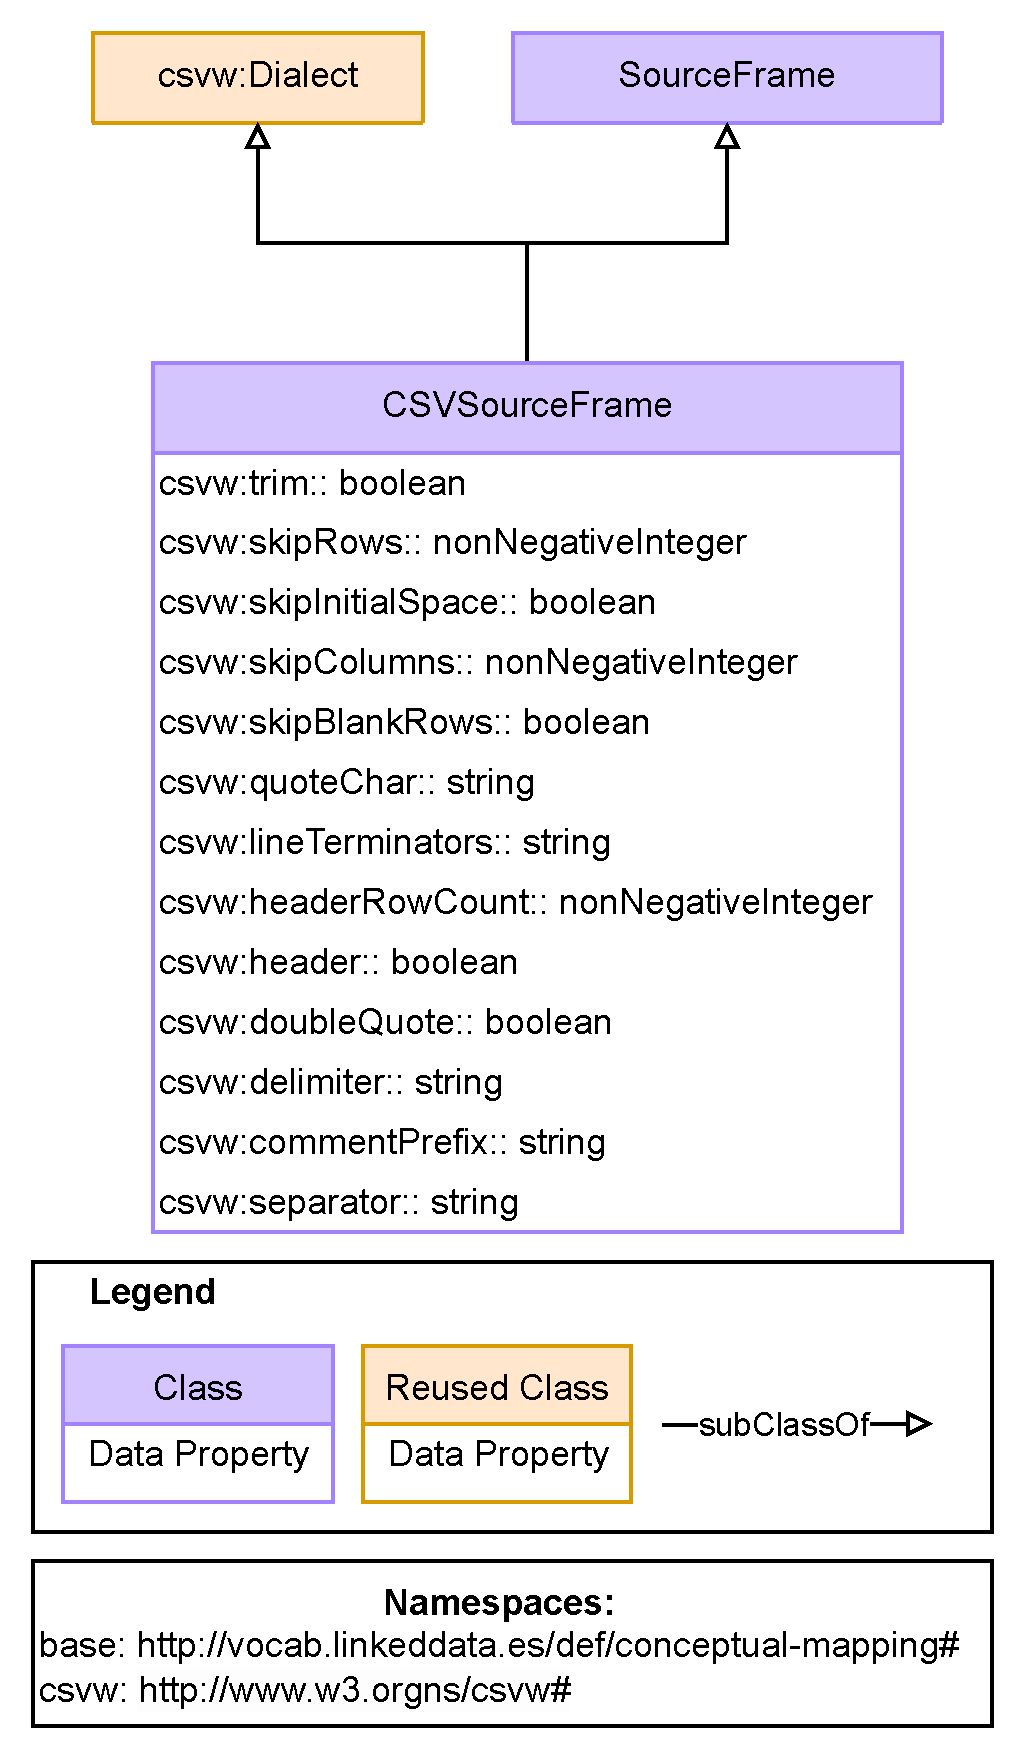
\includegraphics[width=0.5\linewidth]{figures/CSV-extension.pdf}
\caption{CSV extension conceptualization.}
\label{fig:csv-ext}
\end{figure}

\subsubsection{RDF-star generation: CM-star}

RDF-star was recently proposed as an alternative for reification in RDF. It extends the RDF syntax introducing the notion of quoted triples, i.e. triples that can be placed in the position of objects and/or subjects. Since its proposal, it has been increasingly adopted by different semantic technologies. Among them, RML was extended to be able to generate RDF-star graphs~\citep{iglesias2022rmlstar} (further details in \cref{sec:chp4_rml_star}). 



\subsection{Ontology usage example}\label{sec:cm_example} 



\begin{figure}[b!]
    \centering
    \begin{subfigure}[b]{0.45\linewidth}
        \centering
    	\includegraphics[width=1\linewidth]{figures/example_ont}
    	\caption{Example reference ontology that represents the classes \texttt{City} and \texttt{Location}, linked by the property \texttt{eg:location}.}
    	\label{fig:chp4_ex_onto}
    \end{subfigure}
    \begin{subfigure}[b]{0.28\linewidth}
        \centering
    	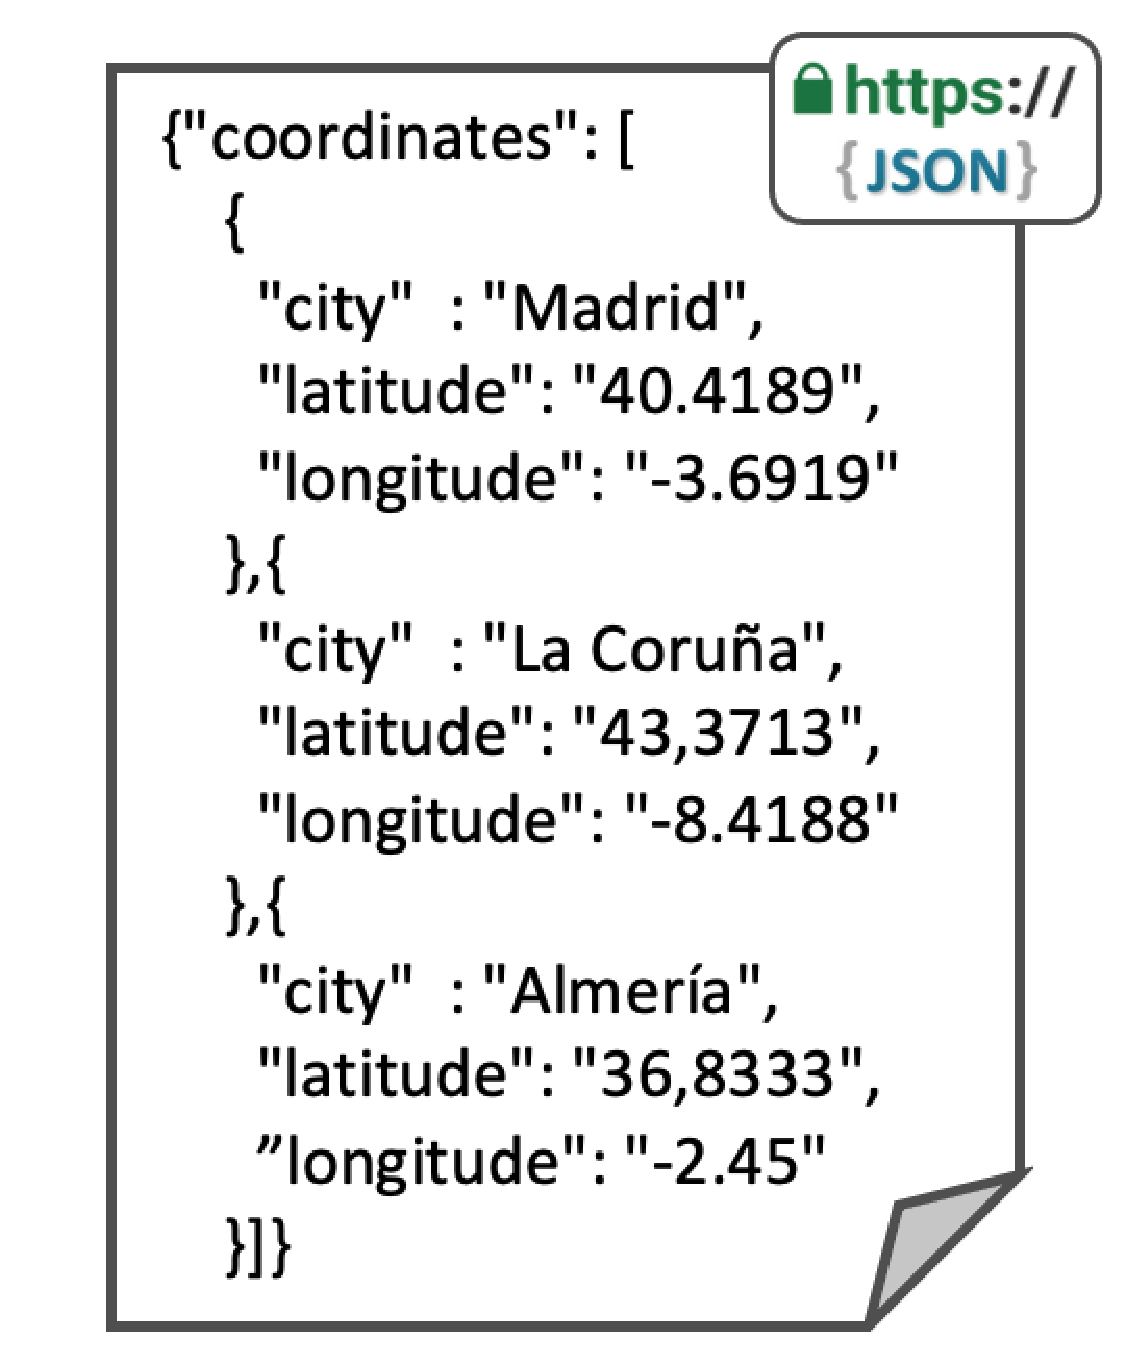
\includegraphics[width=1\linewidth]{figures/example_json}
    	\caption{Example input JSON file ```coordinates.json".}
    	\label{fig:chp4_ex_json}
    \end{subfigure}
    \begin{subfigure}[b]{0.7\linewidth}
        \centering
    	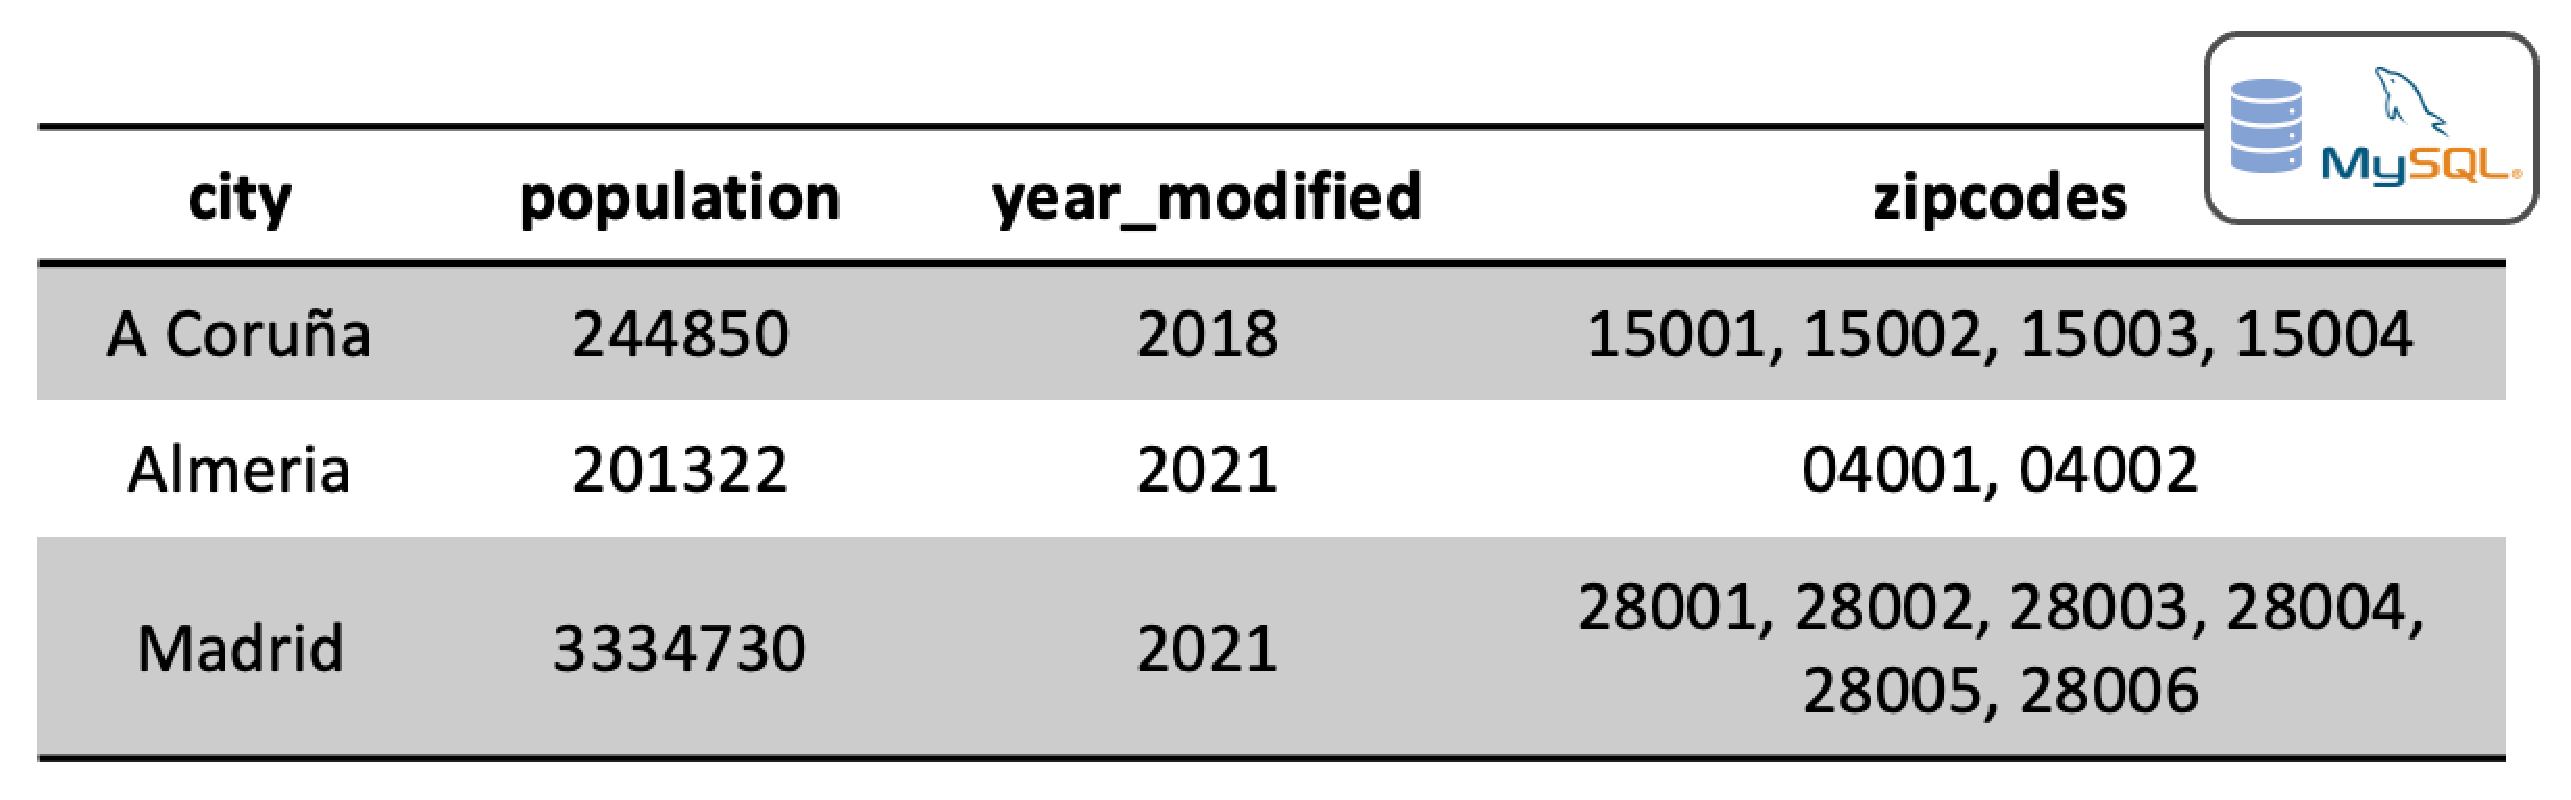
\includegraphics[width=1\linewidth]{figures/example_rdb}
    	\caption{Example input MySQL table ```cities".}
    	\label{fig:chp4_ex_rdb}
    \end{subfigure}
    \caption{Input source data and reference ontology that represents information on cities and their location.}
    \label{fig:chp4_ex_input}
\end{figure}



%\ana{no sé si dejar esto o rehacer y poner de drugs4covid, para que no sean datos de juguete. O si acaso poner que sea un use case, eso requeriría de hacer el mapping también en otros lenguajes. Por ahora dejar como está}

This section builds a mapping in three steps (data sources in \cref{lst:chp4_cm_sources}, triples in \cref{lst:chp4_cm_spo} and special statements in \cref{lst:chp4_cm_general}) to represent how the proposed language can describe data with different features. The mapping uses the data sources ``coordinates.json" (\cref{fig:chp4_ex_json}) and ``cities" (\cref{fig:chp4_ex_rdb}) as input and the ontology depicted in  \cref{fig:chp4_ex_onto} as reference, to create the output RDF shown in \cref{lst:chp4_output}. 
%Additionally, \cref{appendix2}\ana{APENDIX!!} contains a second example to illustrate different features than the ones represented in the example of this section, to provide more insights about the expressiveness of this language.

\begin{captionedlisting}{lst:chp4_output}{Expected RDF output for the data sources and the ontology in \cref{fig:chp4_ex_input}.}
\centering
{\begin{lstlisting}[]
<http://ex.com/loc/40.4189--3.6919> a eg:Location ;
	eg:lat "40.4189"^^xsd:decimal ;
	eg:long "-3.6919"^^xsd:decimal .
<http://ex.com/loc/43.3713--8.4188> a eg:Location ;
	eg:lat "43.3713"^^xsd:decimal ;
	eg:long "-8.4188"^^xsd:decimal .
<http://ex.com/loc/36.8333--2.45> a eg:Location ;
	eg:lat "36.8333"^^xsd:decimal ;
	eg:long "-2.45"^^xsd:decimal .
<http://ex.com/city/ACoruña> a eg:City ;
	eg:zipcode 15001, 15002, 15003, 15004 ;
	eg:location <http://ex.com/loc/43.3713--8.4188> .
<http://ex.com/city/Almería> a eg:City ;
	eg:zipcode 04001, 04002 ;
	eg:population 201322 ;
	eg:location <http://ex.com/loc/36.8333--2.45> .
<http://ex.com/city/Madrid> a eg:City ;
	eg:zipcode 28001, 28002, 28003, 28004, 28005, 28006;
	eg:population 3334730 ;
	eg:location <http://ex.com/loc/40.4189--3.6919> .
\end{lstlisting}}
\end{captionedlisting}

\noindent\paragraph{\textbf{Data sources.}} \cref{lst:chp4_cm_sources} shows the description of the json file ``coordinates.json" indicating the protocol from the SKOS concept scheme (\texttt{cmp:https}), media type (``application/json"), JSONPath to extract data, access URL  ``https://ex.com/geodata/coordi\-nates.json", and  fields that are going to be used in the transformation. There is no security scheme. The MySQL table ``cities" also has no security scheme, the protocol needed is \texttt{cmp:jdbc}, the database access is specified in the endpoint URL, and the table as an SQL query. The fields are also specified, with the special case of ``zipcodes" that needs a \texttt{cm:hasNestedFrame} to extract multiple values inside the field.

\begin{captionedlisting}{lst:chp4_cm_sources}{Description with the Conceptual Mapping of two data sources (a JSON file and a relational database), their access and fields.}
\centering
{\begin{lstlisting}[language=concm,firstnumber=1]
# Locations
:FrameLoc a cm:SourceFrame;
  cm:expression "$\dollar$.coordinates[*]";
  cm:language ql:JSONPath ;
  cm:hasField :lat;
  cm:hasField :long;
  cm:hasField :loc_city;
  cm:hasDataSource [ a cm:SynchronousSource;
    dcat:mediaType "text/json";
    dcat:accessService [
      cm:hasProtocol cmp:https;
      dcat:endpointURL "https://ex.com/geodata/coordinates.json" 
      cm:hasSecurityScheme [ a wotsec:NoSecurityScheme; ];
    ] ;
  ] .

:lat a cm:DataField ; cm:field "$\dollar$.latitude" .
:long a cm:DataField ; cm:field "$\dollar$.longitude" .
:loc_city a cm:DataField; cm:field "$\dollar$.city" .

# Cities
:FrameCities a cm:SourceFrame ;
  cm:expression "SELECT * FROM cities;";
  cm:hasField :c_city;
  cm:hasField :population;
  cm:hasField :year;
  cm:hasNestedFrame [
    cm:expression "$\dollar$.zipcodes[*]";
    cm:hasField :zipcode ];
  cm:hasDataSource [ a cm:SynchronousSource;
    dcat:mediaType "text/plain";
    dcat:accessService [
      cm:hasProtocol cmp:jdbc;
      dcat:endpointURL "jdbc:mysql://localhost:3306/citydb";
      cm:hasSecurityScheme [a wotsec:NoSecurityScheme;] ].

:c_city a cm:DataField; cm:field "city" .
:population a cm:DataField; cm:field "population" .
:year a cm:DataField; cm:field "year_modified" .
:zipcode a cm:DataField cm:field "zipcodes" .
\end{lstlisting}}
\end{captionedlisting}

%\noindent{\textbf{Locations.}} Sarah is working at the National Geographic Institute from Spain, and manages everyday information about places and locations. She wants to create a knowledge graph with the geographical data that she usually manages. She starts writing a mapping (\cref{lst:uc1}) to represent cities from a local JSON file, \texttt{Venue.json} (\cref{lst:data_venues}). This data will be transformed into instances of the class \texttt{City}. 

\noindent\paragraph{\textbf{Statements.}} \cref{lst:chp4_cm_spo} contains the rules needed to create instances of the classes \texttt{eg:Location} and \texttt{eg:City}; and their following attributes: \texttt{eg:lat} and \texttt{eg:long} for the former; \texttt{eg:zipcode} for the latter. To correctly generate the URI for the instances of \texttt{eg:City}, a replace function inside a concatenate function is needed to (1) remove the blank spaces in the field ``city" and (2) add the field to the base URI ``http://ex.com/city/".

\begin{captionedlisting}{lst:chp4_cm_spo}{Description with the Conceptual Mapping of the creation of regular statements from the data sources described in \cref{lst:chp4_cm_sources}.}
\centering
{\begin{lstlisting}[language=concm,firstnumber=1]
# Locations
:SubjectLoc a cm:ReferenceNodeMap ;
  cm:hasEvaluableExpression [
    cm:hasFunctionName cmf:concat; 
    cm:hasInput ([cm:constantValue "http://ex.com/loc/"]    :lat [cm:constantValue "-" ] :long)].

:StatementLoc1 a cm:StatementMap ;
  cm:hasFrame :FrameLoc ;
  cm:subject :SubjectLoc ;
  cm:predicate [ a cm:ReferenceNodeMap; 
    cm:hasEvaluableExpression [cm:constantValue rdf:type ] ];
  cm:object [cm:hasEvaluableExpression [cm:constantValue eg:Location]].

:StatementLoc2 a cm:StatementMap ;
  cm:hasFrame :FrameLoc ;
  cm:subject :SubjectLoc ;
  cm:predicate [ a cm:ReferenceNodeMap; 
    cm:hasEvaluableExpression [cm:constantValue eg:lat]];
  cm:object [ a cm:Literal; cm:hasEvaluableExpression :lat];
  cm:hasDatatype [cm:hasEvaluableExpression xsd:decimal].

:StatementLoc3 a cm:StatementMap ;
  cm:hasFrame :FrameLoc ;
  cm:subject :SubjectLoc ;
  cm:predicate [ a cm:ReferenceNodeMap; 
    cm:hasEvaluableExpression [cm:constantValue eg:long]];
  cm:object [ a cm:Literal; cm:hasEvaluableExpression :long];
  cm:hasDatatype [ cm:hasEvaluableExpression xsd:decimal].
    
# Cities
:city_ns a cm:FunctionExpression ;
  cm:functionName cmf:replace ;
  cm:hasInput (c_city " " "")

:SubjectCities a cm:ReferenceNodeMap;
  cm:hasEvaluableExpression [
    cm:hasFunctionName cmf:concat; 
    cm:hasInput ([cm:constantValue "http://ex.com/city/"] :city_ns)].

:StatementCit1 a cm:StatementMap ;
  cm:hasFrame :FrameCities ;
  cm:subject :SubjectCities ;
  cm:predicate [ a cm:ReferenceNodeMap; 
    cm:hasEvaluableExpression [cm:constantValue rdf:type]];
  cm:object [ a cm:ReferenceNodeMap; 
    cm:hasEvaluableExpression  [cm:constantValue eg:City]] .

:StatementCit2 a cm:StatementMap ;
  cm:hasFrame :FrameCities ;
  cm:subject :SubjectCities ;
  cm:predicate [ a cm:ReferenceNodeMap; 
    cm:hasEvaluableExpression [cm:constantValue rdfs:label]];
  cm:object [ a cm:ReferenceNodeMap; 
    cm:hasEvaluableExpression  [cm:constantValue :c_city]] .
  cm:hasLanguage [ cm:hasEvaluableExpression [ cm:constantValue "es" ] ].

:StatementCit3 a cm:StatementMap ;
  cm:hasFrame :FrameCities ;
  cm:subject :SubjectCities ;
  cm:predicate [ a cm:ReferenceNodeMap; 
    cm:hasEvaluableExpression [cm:constantValue eg:zipcode] ];
  cm:object [ a cm:Literal;
    cm:hasEvaluableExpression [cm:constantValue :zipcode] ];
  cm:hasDatatype [ cm:hasEvaluableExpression xsd:integer ].
\end{lstlisting}}
\end{captionedlisting}


\noindent\paragraph{\textbf{Special statements.}} \cref{lst:chp4_cm_general} describes how a conditional statement and a linking rule are generated. This description is represented by means of functions. With the property \texttt{cm:hasBooleanCondition}, the conditional statement declares that the field \texttt{:year} has to be greater than 2020. The linking rule performs the link between the instances of \texttt{eg:City} and \texttt{eg:Location} with the predicate \texttt{eg:location}, using a distance metric (levenshtein function) that has to be greater then a threshold of ``0.75". 

\begin{captionedlisting}{lst:chp4_cm_general}{Conditional and linking rules described with the Conceptual Mapping that complement the data source description and regular statements described in \cref{lst:chp4_cm_sources} and \cref{lst:chp4_cm_spo}.}
\centering
{\begin{lstlisting}[language=concm,firstnumber=1]
:StatementCit4 a cm:ConditionalStatementMap ;
  cm:hasFrame :FrameCities ;
  cm:subject :SubjectCities ;
  cm:predicate [ a cm:ReferenceNodeMap; 
    cm:hasEvaluableExpression [cm:constantValue eg:population] ];
  cm:object [ a cm:Literal; 
    cm:hasEvaluableExpression  [cm:constantValue :population] ];
  cm:hasDatatype [ cm:hasEvaluableExpression xsd:integer];
  cm:hasBooleanCondition [
    cm:functionName cmf:greater_than ;
    cm:hasInput ( :year 2020 ) ] .

:LinkExp1 a cm:LinkingExpression ;
  cm:source :StatementCit1 ;
  cm:target :StatementLoc1 ;
  cm:property eg:location ;
  cm:hasBooleanCondition [
    cm:functionName cmf:greater_than ; 
    cm:hasInput ( :levfun 0.75 ) ] .

:levfun a cm:FunctionExpression ;
  cm:functionName cmf:levenshtein_distance ;    
  cm:hasInput (:c_city :loc_city) .
\end{lstlisting}}
\end{captionedlisting}







